%%
% Copyright (c) 2017 - 2019, Pascal Wagler;  
% Copyright (c) 2014 - 2019, John MacFarlane
% 
% All rights reserved.
% 
% Redistribution and use in source and binary forms, with or without 
% modification, are permitted provided that the following conditions 
% are met:
% 
% - Redistributions of source code must retain the above copyright 
% notice, this list of conditions and the following disclaimer.
% 
% - Redistributions in binary form must reproduce the above copyright 
% notice, this list of conditions and the following disclaimer in the 
% documentation and/or other materials provided with the distribution.
% 
% - Neither the name of John MacFarlane nor the names of other 
% contributors may be used to endorse or promote products derived 
% from this software without specific prior written permission.
% 
% THIS SOFTWARE IS PROVIDED BY THE COPYRIGHT HOLDERS AND CONTRIBUTORS 
% "AS IS" AND ANY EXPRESS OR IMPLIED WARRANTIES, INCLUDING, BUT NOT 
% LIMITED TO, THE IMPLIED WARRANTIES OF MERCHANTABILITY AND FITNESS 
% FOR A PARTICULAR PURPOSE ARE DISCLAIMED. IN NO EVENT SHALL THE 
% COPYRIGHT OWNER OR CONTRIBUTORS BE LIABLE FOR ANY DIRECT, INDIRECT, 
% INCIDENTAL, SPECIAL, EXEMPLARY, OR CONSEQUENTIAL DAMAGES (INCLUDING,
% BUT NOT LIMITED TO, PROCUREMENT OF SUBSTITUTE GOODS OR SERVICES; 
% LOSS OF USE, DATA, OR PROFITS; OR BUSINESS INTERRUPTION) HOWEVER 
% CAUSED AND ON ANY THEORY OF LIABILITY, WHETHER IN CONTRACT, STRICT 
% LIABILITY, OR TORT (INCLUDING NEGLIGENCE OR OTHERWISE) ARISING IN 
% ANY WAY OUT OF THE USE OF THIS SOFTWARE, EVEN IF ADVISED OF THE 
% POSSIBILITY OF SUCH DAMAGE.
%%

%%
% This is the Eisvogel pandoc LaTeX template.
%
% For usage information and examples visit the official GitHub page:
% https://github.com/Wandmalfarbe/pandoc-latex-template
%%

\PassOptionsToPackage{unicode=true}{hyperref} % options for packages loaded elsewhere
\PassOptionsToPackage{hyphens}{url}
\PassOptionsToPackage{dvipsnames,svgnames*,x11names*,table}{xcolor}
%
\documentclass[
  10pt,
  english,
  letterpaper,
,tablecaptionabove
]{scrartcl}
\usepackage{lmodern}
\usepackage{setspace}
\setstretch{1.2}
\usepackage{amssymb,amsmath}
\usepackage{ifxetex,ifluatex}
\ifnum 0\ifxetex 1\fi\ifluatex 1\fi=0 % if pdftex
  \usepackage[T1]{fontenc}
  \usepackage[utf8]{inputenc}
  \usepackage{textcomp} % provides euro and other symbols
\else % if luatex or xelatex
  \usepackage{unicode-math}
  \defaultfontfeatures{Scale=MatchLowercase}
  \defaultfontfeatures[\rmfamily]{Ligatures=TeX,Scale=1}
\fi
% use upquote if available, for straight quotes in verbatim environments
\IfFileExists{upquote.sty}{\usepackage{upquote}}{}
\IfFileExists{microtype.sty}{% use microtype if available
  \usepackage[]{microtype}
  \UseMicrotypeSet[protrusion]{basicmath} % disable protrusion for tt fonts
}{}
\makeatletter
\@ifundefined{KOMAClassName}{% if non-KOMA class
  \IfFileExists{parskip.sty}{%
    \usepackage{parskip}
  }{% else
    \setlength{\parindent}{0pt}
    \setlength{\parskip}{6pt plus 2pt minus 1pt}}
}{% if KOMA class
  \KOMAoptions{parskip=half}}
\makeatother
\usepackage{xcolor}
\definecolor{default-linkcolor}{HTML}{A50000}
\definecolor{default-filecolor}{HTML}{A50000}
\definecolor{default-citecolor}{HTML}{4077C0}
\definecolor{default-urlcolor}{HTML}{4077C0}
\IfFileExists{xurl.sty}{\usepackage{xurl}}{} % add URL line breaks if available
\IfFileExists{bookmark.sty}{\usepackage{bookmark}}{\usepackage{hyperref}}
\hypersetup{
  pdftitle={Red-Black Trees (Part 1)},
  pdfauthor={Connor Baker},
  pdfsubject={Red-Black Trees},
  pdfkeywords={Lecture, Red-Black, Self-Balancing Trees},
  pdfborder={0 0 0},
  breaklinks=true}
\urlstyle{same}  % don't use monospace font for urls
\usepackage[margin=2.5cm,includehead=true,includefoot=true,centering]{geometry}
\usepackage{listings}
\newcommand{\passthrough}[1]{#1}
\lstset{defaultdialect=[5.3]Lua}
\lstset{defaultdialect=[x86masm]Assembler}
\usepackage{graphicx,grffile}
\makeatletter
\def\maxwidth{\ifdim\Gin@nat@width>\linewidth\linewidth\else\Gin@nat@width\fi}
\def\maxheight{\ifdim\Gin@nat@height>\textheight\textheight\else\Gin@nat@height\fi}
\makeatother
% Scale images if necessary, so that they will not overflow the page
% margins by default, and it is still possible to overwrite the defaults
% using explicit options in \includegraphics[width, height, ...]{}
\setkeys{Gin}{width=\maxwidth,height=\maxheight,keepaspectratio}
\setlength{\emergencystretch}{3em}  % prevent overfull lines
\providecommand{\tightlist}{%
  \setlength{\itemsep}{0pt}\setlength{\parskip}{0pt}}
\setcounter{secnumdepth}{-\maxdimen} % remove section numbering
% Redefines (sub)paragraphs to behave more like sections
\ifx\paragraph\undefined\else
  \let\oldparagraph\paragraph
  \renewcommand{\paragraph}[1]{\oldparagraph{#1}\mbox{}}
\fi
\ifx\subparagraph\undefined\else
  \let\oldsubparagraph\subparagraph
  \renewcommand{\subparagraph}[1]{\oldsubparagraph{#1}\mbox{}}
\fi

% Make use of float-package and set default placement for figures to H
\usepackage{float}
\floatplacement{figure}{H}

\setcounter{page}{0}
\lstset{breaklines=true}
\lstset{postbreak=\raisebox{0ex}[0ex][0ex]{\ensuremath{\color{blue}\hookrightarrow\space}}}
\usepackage{datetime}
\settimeformat{ampmtime}
\usepackage{lastpage}
\ifnum 0\ifxetex 1\fi=0 % if pdftex or luatex
  \usepackage[shorthands=off,main=english]{babel}
\else % if xetex
    % See issue https://github.com/reutenauer/polyglossia/issues/127
  \renewcommand*\familydefault{\sfdefault}
    % load polyglossia as late as possible as it *could* call bidi if RTL lang (e.g. Hebrew or Arabic)
  \usepackage{polyglossia}
  \setmainlanguage[]{english}
\fi

\title{Red-Black Trees (Part 1)}
\usepackage{etoolbox}
\makeatletter
\providecommand{\subtitle}[1]{% add subtitle to \maketitle
  \apptocmd{\@title}{\par {\large #1 \par}}{}{}
}
\makeatother
\subtitle{Red-black trees and their rotation cases}
\author{Connor Baker}
\date{2019-04-15, Compiled on \today~at \currenttime}





%%
%% added
%%

%
% language specification
%
% If no language is specified, use English as the default main document language.
%


%
% for the background color of the title page
%
\usepackage{pagecolor}
\usepackage{afterpage}

%
% TOC depth and 
% section numbering depth
%
\setcounter{tocdepth}{3}

%
% break urls
%
\PassOptionsToPackage{hyphens}{url}

%
% When using babel or polyglossia with biblatex, loading csquotes is recommended 
% to ensure that quoted texts are typeset according to the rules of your main language.
%
\usepackage{csquotes}

%
% captions
%
\definecolor{caption-color}{HTML}{777777}
\usepackage[font={stretch=1.2}, textfont={color=caption-color}, position=top, skip=4mm, labelfont=bf, singlelinecheck=false, justification=raggedright]{caption}
\setcapindent{0em}

%
% blockquote
%
\definecolor{blockquote-border}{RGB}{221,221,221}
\definecolor{blockquote-text}{RGB}{119,119,119}
\usepackage{mdframed}
\newmdenv[rightline=false,bottomline=false,topline=false,linewidth=3pt,linecolor=blockquote-border,skipabove=\parskip]{customblockquote}
\renewenvironment{quote}{\begin{customblockquote}\list{}{\rightmargin=0em\leftmargin=0em}%
\item\relax\color{blockquote-text}\ignorespaces}{\unskip\unskip\endlist\end{customblockquote}}

%
% Source Sans Pro as the de­fault font fam­ily
% Source Code Pro for monospace text
%
% 'default' option sets the default 
% font family to Source Sans Pro, not \sfdefault.
%
\usepackage[default]{sourcesanspro}
\usepackage{sourcecodepro}

% XeLaTeX specific adjustments for straight quotes: https://tex.stackexchange.com/a/354887
% This issue is already fixed (see https://github.com/silkeh/latex-sourcecodepro/pull/5) but the 
% fix is still unreleased.
% TODO: Remove this workaround when the new version of sourcecodepro is released on CTAN.
\ifxetex
\makeatletter
\defaultfontfeatures[\ttfamily]
  { Numbers   = \sourcecodepro@figurestyle,
    Scale     = \SourceCodePro@scale,
    Extension = .otf }
\setmonofont
  [ UprightFont    = *-\sourcecodepro@regstyle,
    ItalicFont     = *-\sourcecodepro@regstyle It,
    BoldFont       = *-\sourcecodepro@boldstyle,
    BoldItalicFont = *-\sourcecodepro@boldstyle It ]
  {SourceCodePro}
\makeatother
\fi

%
% heading color
%
\definecolor{heading-color}{RGB}{40,40,40}
\addtokomafont{section}{\color{heading-color}}
% When using the classes report, scrreprt, book, 
% scrbook or memoir, uncomment the following line.
%\addtokomafont{chapter}{\color{heading-color}}

%
% variables for title and author
%
\usepackage{titling}
\title{Red-Black Trees (Part 1)}
\author{Connor Baker}

%
% tables
%

%
% remove paragraph indention
%
\setlength{\parindent}{0pt}
\setlength{\parskip}{6pt plus 2pt minus 1pt}
\setlength{\emergencystretch}{3em}  % prevent overfull lines

%
%
% Listings
%
%


%
% listing colors
%
\definecolor{listing-background}{HTML}{F7F7F7}
\definecolor{listing-rule}{HTML}{B3B2B3}
\definecolor{listing-numbers}{HTML}{B3B2B3}
\definecolor{listing-text-color}{HTML}{000000}
\definecolor{listing-keyword}{HTML}{435489}
\definecolor{listing-identifier}{HTML}{435489}
\definecolor{listing-string}{HTML}{00999A}
\definecolor{listing-comment}{HTML}{8E8E8E}
\definecolor{listing-javadoc-comment}{HTML}{006CA9}

\lstdefinestyle{eisvogel_listing_style}{
  language         = java,
  numbers          = left,
  xleftmargin      = 2.7em,
  framexleftmargin = 2.5em,
  backgroundcolor  = \color{listing-background},
  basicstyle       = \color{listing-text-color}\small\ttfamily{}\linespread{1.15}, % print whole listing small
  breaklines       = true,
  frame            = single,
  framesep         = 0.19em,
  rulecolor        = \color{listing-rule},
  frameround       = ffff,
  tabsize          = 4,
  numberstyle      = \color{listing-numbers},
  aboveskip        = -0.7em,
  belowskip        = 0.1em,
  abovecaptionskip = 0em,
  belowcaptionskip = 1em,
  keywordstyle     = \color{listing-keyword}\bfseries,
  classoffset      = 0,
  sensitive        = true,
  identifierstyle  = \color{listing-identifier},
  commentstyle     = \color{listing-comment},
  morecomment      = [s][\color{listing-javadoc-comment}]{/**}{*/},
  stringstyle      = \color{listing-string},
  showstringspaces = false,
  escapeinside     = {/*@}{@*/}, % Allow LaTeX inside these special comments
  literate         =
  {á}{{\'a}}1 {é}{{\'e}}1 {í}{{\'i}}1 {ó}{{\'o}}1 {ú}{{\'u}}1
  {Á}{{\'A}}1 {É}{{\'E}}1 {Í}{{\'I}}1 {Ó}{{\'O}}1 {Ú}{{\'U}}1
  {à}{{\`a}}1 {è}{{\'e}}1 {ì}{{\`i}}1 {ò}{{\`o}}1 {ù}{{\`u}}1
  {À}{{\`A}}1 {È}{{\'E}}1 {Ì}{{\`I}}1 {Ò}{{\`O}}1 {Ù}{{\`U}}1
  {ä}{{\"a}}1 {ë}{{\"e}}1 {ï}{{\"i}}1 {ö}{{\"o}}1 {ü}{{\"u}}1
  {Ä}{{\"A}}1 {Ë}{{\"E}}1 {Ï}{{\"I}}1 {Ö}{{\"O}}1 {Ü}{{\"U}}1
  {â}{{\^a}}1 {ê}{{\^e}}1 {î}{{\^i}}1 {ô}{{\^o}}1 {û}{{\^u}}1
  {Â}{{\^A}}1 {Ê}{{\^E}}1 {Î}{{\^I}}1 {Ô}{{\^O}}1 {Û}{{\^U}}1
  {œ}{{\oe}}1 {Œ}{{\OE}}1 {æ}{{\ae}}1 {Æ}{{\AE}}1 {ß}{{\ss}}1
  {ç}{{\c c}}1 {Ç}{{\c C}}1 {ø}{{\o}}1 {å}{{\r a}}1 {Å}{{\r A}}1
  {€}{{\EUR}}1 {£}{{\pounds}}1 {«}{{\guillemotleft}}1
  {»}{{\guillemotright}}1 {ñ}{{\~n}}1 {Ñ}{{\~N}}1 {¿}{{?`}}1
  {…}{{\ldots}}1 {≥}{{>=}}1 {≤}{{<=}}1 {„}{{\glqq}}1 {“}{{\grqq}}1
  {”}{{''}}1
}
\lstset{style=eisvogel_listing_style}

\lstdefinelanguage{XML}{
  morestring      = [b]",
  moredelim       = [s][\bfseries\color{listing-keyword}]{<}{\ },
  moredelim       = [s][\bfseries\color{listing-keyword}]{</}{>},
  moredelim       = [l][\bfseries\color{listing-keyword}]{/>},
  moredelim       = [l][\bfseries\color{listing-keyword}]{>},
  morecomment     = [s]{<?}{?>},
  morecomment     = [s]{<!--}{-->},
  commentstyle    = \color{listing-comment},
  stringstyle     = \color{listing-string},
  identifierstyle = \color{listing-identifier}
}

%
% header and footer
%
\usepackage{fancyhdr}

\fancypagestyle{eisvogel-header-footer}{
  \fancyhead{}
  \fancyfoot{}
  \lhead[2019-04-15]{Red-Black Trees (Part 1)}
  \chead[]{}
  \rhead[Red-Black Trees (Part 1)]{2019-04-15}
  \lfoot[\thepage~of \pageref{LastPage}]{Connor Baker}
  \cfoot[]{}
  \rfoot[Connor Baker]{\thepage~of \pageref{LastPage}}
  \renewcommand{\headrulewidth}{0.4pt}
  \renewcommand{\footrulewidth}{0.4pt}
}
\pagestyle{eisvogel-header-footer}

%%
%% end added
%%

\begin{document}

%%
%% begin titlepage
%%

\begin{titlepage}
\newgeometry{left=6cm}
\definecolor{titlepage-color}{HTML}{FFFFFF}
\newpagecolor{titlepage-color}\afterpage{\restorepagecolor}
\newcommand{\colorRule}[3][black]{\textcolor[HTML]{#1}{\rule{#2}{#3}}}
\begin{flushleft}
\noindent
\\[-1em]
\color[HTML]{0d47a1}
\makebox[0pt][l]{\colorRule[0d47a1]{1.3\textwidth}{2pt}}
\par
\noindent

{ \setstretch{1.4}
\vfill
\noindent {\huge \textbf{\textsf{Red-Black Trees (Part 1)}}}
\vskip 1em
{\Large \textsf{Red-black trees and their rotation cases}}
\vskip 2em
\noindent
{\Large \textsf{Connor Baker}
\vfill
}


\textsf{2019-04-15, Compiled on \today~at \currenttime}}
\end{flushleft}
\end{titlepage}
\restoregeometry

%%
%% end titlepage
%%



\hypertarget{red-black-trees-part-1}{%
\section{Red-Black Trees (Part 1)}\label{red-black-trees-part-1}}

\hypertarget{review}{%
\subsection{Review}\label{review}}

\begin{itemize}
\tightlist
\item
  Binary search tree with self-balancing features

  \begin{itemize}
  \tightlist
  \item
    AVL trees

    \begin{itemize}
    \tightlist
    \item
      Definition: binary search tree with a balanced height
    \item
      Operation and analysis

      \begin{itemize}
      \tightlist
      \item
        Single or double rotations
      \end{itemize}
    \end{itemize}
  \end{itemize}
\end{itemize}

\hypertarget{red-black-trees}{%
\subsection{Red-Black Trees}\label{red-black-trees}}

\begin{itemize}
\tightlist
\item
  In a 1978 paper \enquote{A Dichromatic Framework for Balanced Trees},
  Leonidas J. Guibas and Robert Sedgewick derived red-black tree from
  symmetric binary B-tree. The color \enquote{red} was chosen because it
  was the best-looking color produced by the color laser printer.."
  (Wikipedia:Red-black tree)
\item
  Could perform insertion in a single top-down pass

  \begin{itemize}
  \tightlist
  \item
    AVL trees require one pass down for insertion, and a second pass
    upwards to update the height and re-balance
  \end{itemize}
\item
  Red-black trees

  \begin{itemize}
  \tightlist
  \item
    Definition: four features
  \item
    Operation: insertion
  \item
    Analysis: how can we ensure a height of \(\log(N)\)?
  \end{itemize}
\end{itemize}

\hypertarget{red-black-tree-definition}{%
\subsection{Red-Black Tree Definition}\label{red-black-tree-definition}}

\begin{itemize}
\tightlist
\item
  A binary search tree with four additional properties

  \begin{enumerate}
  \def\labelenumi{\arabic{enumi}.}
  \tightlist
  \item
    Every node is either red or black
  \item
    The root is black
  \item
    If a node is red, its children are black -- the converse is
    \emph{not necessarily true}
  \item
    Every path from the root to \passthrough{\lstinline!null!} has the
    same number of black nodes
  \end{enumerate}
\end{itemize}

\hypertarget{red-black-trees-vs-avl-trees}{%
\subsection{Red-Black Trees vs AVL
Trees}\label{red-black-trees-vs-avl-trees}}

\begin{itemize}
\tightlist
\item
  Both are special binary search trees
\end{itemize}

\begin{figure}
\centering
\includegraphics[width=0.25\textwidth,height=\textheight]{images/1.png}
\caption{Example one}
\end{figure}

\begin{itemize}
\tightlist
\item
  Is this a red-black tree?

  \begin{itemize}
  \tightlist
  \item
    Yes:

    \begin{enumerate}
    \def\labelenumi{\arabic{enumi}.}
    \tightlist
    \item
      Every node is either red or black
    \item
      The root is black
    \item
      If a node is red, its children are black
    \item
      Every path from the root to \passthrough{\lstinline!null!} has the
      same number of black nodes: 1
    \end{enumerate}
  \end{itemize}
\item
  Is this an AVL tree?

  \begin{itemize}
  \tightlist
  \item
    No, because there is a difference of more than one between the left
    and right subtrees
  \end{itemize}
\end{itemize}

\hypertarget{insertion-basics}{%
\subsection{Insertion Basics}\label{insertion-basics}}

\begin{itemize}
\tightlist
\item
  Implementations tend to use recursion for clarity (though it's still
  more complicated than the implementation for insertion in an AVL tree)
\item
  Insert data as if it were a normal binary search tree

  \begin{itemize}
  \tightlist
  \item
    Color the new node red and insert it as a leaf \textbf{(why red?)}
  \item
    If this creates two adjacent red nodes, fix it
  \item
    Fix all red-red child-parent pairs using rotations or recolors
  \end{itemize}
\end{itemize}

\hypertarget{easy-case}{%
\subsection{Easy Case}\label{easy-case}}

\begin{figure}
\centering
\includegraphics[width=0.25\textwidth,height=\textheight]{images/1.png}
\caption{Insertion with an easy case}
\end{figure}

\begin{itemize}
\tightlist
\item
  Inserting \(110\) or \(211\)

  \begin{itemize}
  \tightlist
  \item
    With a black parent node: easy
  \item
    No two adjacent red nodes
  \item
    The same black depth for all nodes with a
    \passthrough{\lstinline!null!}-child including the new node
  \item
    Black depth of a node: the number of black nodes from root to that
    node
  \end{itemize}
\end{itemize}

\hypertarget{recolor-case}{%
\subsection{Recolor Case}\label{recolor-case}}

\begin{figure}
\centering
\includegraphics[width=0.5\textwidth,height=\textheight]{images/2.png}
\caption{Insertion pre-recoloring}
\end{figure}

\begin{itemize}
\tightlist
\item
  Inserting \(262\)

  \begin{itemize}
  \tightlist
  \item
    The new node has a red parent and a red uncle (they are \emph{not}
    \passthrough{\lstinline!null!})
  \item
    Grandparent must be black
  \item
    Recolor the grandparent, parent, and uncle (red-black-black)

    \begin{itemize}
    \tightlist
    \item
      After this point, we'll need to check the grandparent and make
      sure that we haven't messed up the supertree
    \end{itemize}
  \end{itemize}
\end{itemize}

\begin{figure}
\centering
\includegraphics[width=0.5\textwidth,height=\textheight]{images/3.png}
\caption{Insertion post-recoloring}
\end{figure}

\hypertarget{recolor-up-the-tree}{%
\subsection{Recolor Up the Tree}\label{recolor-up-the-tree}}

\begin{itemize}
\tightlist
\item
  The general case of a red parent and red uncle:

  \begin{itemize}
  \tightlist
  \item
    After recoloring, the grandparent becomes red and might conflict
    with the newly inserted node's red great-grandparent
  \end{itemize}
\end{itemize}

\begin{figure}
\centering
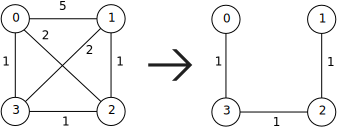
\includegraphics[width=0.75\textwidth,height=\textheight]{images/4.png}
\caption{Recoloring the tree}
\end{figure}

\hypertarget{rotation-case}{%
\subsection{Rotation Case}\label{rotation-case}}

\begin{figure}
\centering
\includegraphics[width=0.35\textwidth,height=\textheight]{images/5.png}
\caption{Insertion with a case involving rotation}
\end{figure}

\begin{itemize}
\tightlist
\item
  Insert \(105\)

  \begin{itemize}
  \tightlist
  \item
    New node with a red parent and a black uncle

    \begin{itemize}
    \tightlist
    \item
      The \passthrough{\lstinline!null!} child of \(112\) is considered
      black
    \end{itemize}
  \item
    Can we recolor the grandparent to red and the parent to black?

    \begin{itemize}
    \tightlist
    \item
      Nope!
    \item
      The \passthrough{\lstinline!null!} child of \(112\) would have a
      changed black depth!
    \end{itemize}
  \item
    Then we must use a rotation and a recolor

    \begin{itemize}
    \tightlist
    \item
      Right-rotate \(110\) recoloring it black, and recolor \(112\) as
      red
    \end{itemize}
  \end{itemize}
\end{itemize}

\begin{figure}
\centering
\includegraphics[width=0.4\textwidth,height=\textheight]{images/6.png}
\caption{Tree after rotation and recoloring}
\end{figure}

\hypertarget{rotation-general-cases}{%
\subsection{Rotation General Cases}\label{rotation-general-cases}}

\begin{itemize}
\tightlist
\item
  The new node is red, the parent is red, and the uncle is black

  \begin{itemize}
  \tightlist
  \item
    Note: more black on the uncle's side of the tree
  \end{itemize}
\item
  Step 1: perform a rotation at the parent \emph{if needed}

  \begin{itemize}
  \tightlist
  \item
    \textbf{When do we do this? Why?}
  \end{itemize}
\end{itemize}

\begin{figure}
\centering
\includegraphics[width=0.75\textwidth,height=\textheight]{images/7.png}
\caption{Step 1}
\end{figure}

\begin{itemize}
\tightlist
\item
  Step 2: perform a rotation at the grandparent
\item
  Step 3: swap the old parent and the grandparent's colors
\end{itemize}

\begin{figure}
\centering
\includegraphics[width=0.75\textwidth,height=\textheight]{images/8.png}
\caption{Steps 2 and 3}
\end{figure}

\hypertarget{red-black-tree-insertion-notes}{%
\subsection{Red-Black Tree Insertion
Notes}\label{red-black-tree-insertion-notes}}

\begin{itemize}
\tightlist
\item
  Cases have mirror cases (the right side cases are all mirrors of the
  left side which we've already discussed)

  \begin{itemize}
  \tightlist
  \item
    Before you ask: cases don't have an agreed upon numbering
  \end{itemize}
\item
  Use the Gnarley Trees demo (\passthrough{\lstinline!gt.jar!}) to play
  around with the trees
\end{itemize}

\end{document}
